% -----------------------------------------------------------------------------
%   Arquivo: ./02-elementos-textuais/trabalhosRelacionados.tex
% -----------------------------------------------------------------------------

\chapter{Aprendizado de Máquina}
\label{chap:MachineLearning}

Nos primórdios da inteligência artificial, pesquisadores foram capazes de resolver problemas que são intelectualmente difíceis para os seres humanos, mas relativamente simples para os computadores. Como problemas que podem ser descritos por uma sequência de regras ou que podem ser solucionados por operações matemáticas. A dificuldade para os computadores foi resolver tarefas que são fáceis para os humanos, mas difíceis de serem descritas de forma algorítmica.  Como reconhecer escrita, identificar rostos em imagens ou ainda definir regras de decisão.

Eis que surgiu o campo de Aprendizado Máquina, como uma alternativa que permitia computadores aprender por exemplo e não por regras ou modelagem matemática. Ao reunir o conhecimento da experiência, esta abordagem evita a necessidade de operadores humanos especificar formalmente todo o conhecimento que o computador precisa. Isso ocorre através da combinação do aprendizado de conceitos simples, em formato pré-definido, combinados de forma hierárquica para formar um aprendizado de conceitos complicados.

O Aprendizado de Máquinas clássico diz respeito à aprender por exemplo, que é definido como um conjunto de dados, previamente obtido, composto por variáveis quantitativas e qualitativas que são características do problema. Na situação onde existe uma variável resposta, o aprendizado é chamado de supervisionado, na situação onde essa variável não existe, o problema é definido como aprendizado não supervisionado. A figura \ref{fig:MLProblems} ilustra essa taxonomia, bem como algumas de suas sub-divisões.


\begin{figure}[!htb]
	\centering
	\caption{Problemas de Aprendizado de Máquina} 
	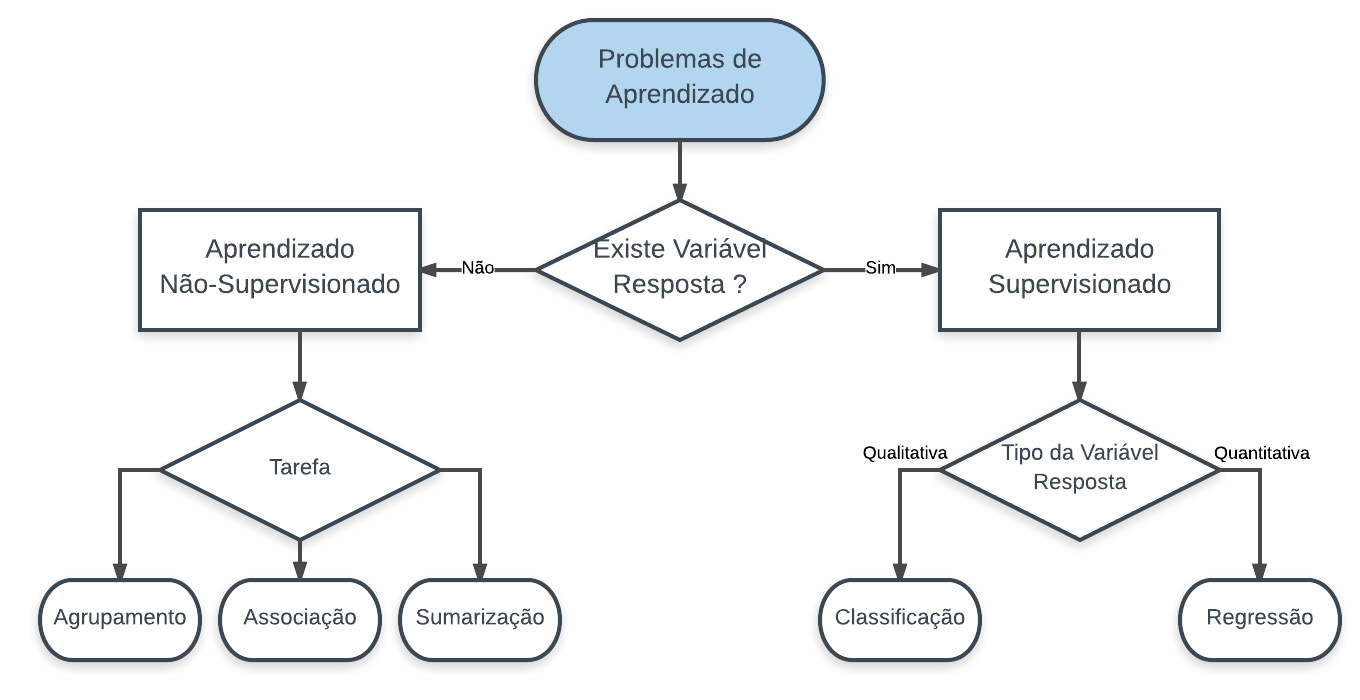
\includegraphics[width=0.8\textwidth]{./04-figuras/MLProblems.png}
	\label{fig:MLProblems}
\end{figure}

\section{Aprendizado Supervisionado}

No aprendizado supervisionado, o objetivo é prever o valor de uma variável resultado com base em variáveis características. Na situação que a variável resposta é quantitativa, o problema é considerado como uma tarefa de regressão. Quando essa variável resposta é quantitativa, a tarefa é chamada de classificação.

\subsection{Problemas de Classificação}
\subsection{Problemas de Regressão}

\section{Aprendizado Não Supervisionado}

\section{Métricas de Aprendizado}
